\documentclass[tikz,border=1pt]{standalone}
\usepackage{tikz}

\tikzset{every node/.style={shape=circle,draw = black}}
\tikzset{every edge/.style={draw = red, very thick}}
\begin{document}
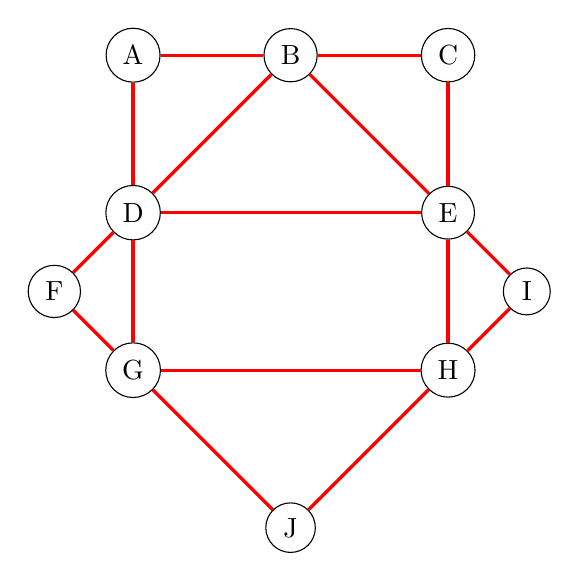
\begin{tikzpicture}[node distance = 2cm]
  \node (A) {A};
  \node (B) [right of= A] {B};
  \node (C) [right of = B] {C};
  \node (D) [below of = A] {D};
  \node (E) [below of = C] {E};
  \node (F) [node distance = 1cm, below of = D, left of = D] {F};
  \node (G) [below of = D] {G};
  \node (H) [below of = E] {H};
  \node (I) [node distance = 1cm, below of = E, right of = E] {I};
  \node (J) [below of = G, right of = G] {J};

  \path (A) edge (B);
  \path (A) edge (D);

  \path (B) edge (C);
  \path (B) edge (D);
  \path (B) edge (E);

  \path (C) edge (E);

  \path (D) edge (E);
  \path (D) edge (F);
  \path (D) edge (G);

  \path (E) edge (H);
  \path (E) edge (I);

  \path (F) edge (G);

  \path (G) edge (H);
  \path (G) edge (J);

  \path (H) edge (I);
  \path (H) edge (J);
\end{tikzpicture}

\end{document}
